\documentclass[conference]{IEEEtran}
\IEEEoverridecommandlockouts
% The preceding line is only needed to identify funding in the first footnote. If that is unneeded, please comment it out.
\usepackage{cite}
\usepackage{amsmath,amssymb,amsfonts}
\usepackage{algorithmic}
\usepackage{graphicx}
\usepackage{subfigure}
\usepackage{float}
\usepackage{textcomp}
\def\BibTeX{{\rm B\kern-.05em{\sc i\kern-.025em b}\kern-.08em
    T\kern-.1667em\lower.7ex\hbox{E}\kern-.125emX}}
\DeclareMathOperator*{\argmax}{argmax}
\usepackage{algorithm} % 伪代码	
\usepackage{algorithmic}  %伪代码
\renewcommand{\algorithmicrequire}{\textbf{Input:}} 
\renewcommand{\algorithmicensure}{\textbf{Output:}}
    
\begin{document}

\title{An Image Classification Algorithm based on AdaBoost and Different Feature Extraction Methods\\
}

\author{\IEEEauthorblockN{Mengfan Wang}
\IEEEauthorblockA{The Bradley Department of Electrical\\ and Computer Engineering\\
Virginia Tech\\
Blacksburg, VA \\
Email: mengfanw@vt.edu}
\and
\IEEEauthorblockN{Yuxian Ye}
\IEEEauthorblockA{The Bradley Department of Electrical\\ and Computer Engineering\\
Virginia Tech\\
Blacksburg, VA \\
Email: herexian@vt.edu}
}

\maketitle

\begin{abstract}
This proposal presents a new image classification method based on three kinds of image feature extraction algorithms, SIFT, LBP, and HOG. They are involved jointly to enhance their advantages. SIFT feature points are reduced to 40 dimensions by PCA to decrease the requirement of computation, and then divided to different clusters by K-means. All of the three features are converted to histogram vectors and be classified by one-versus-all SVM. The finial classifier combines the three weak classifiers by AdaBoost, and is generalized by 5-fold cross-validation.
\end{abstract}

\begin{IEEEkeywords}
image classifier, SIFT, LBP, HOG, PCA, bag of words, K-means, SVM, AdaBoost 
\end{IEEEkeywords}

\section{Introduction}The development of computer vision technology gives birth to more and more feature extraction algorithms. These algorithms have different advantages and disadvantages and are applied in many areas. For example, features extracted by SIFT\cite{sift} include rotation, illumination, scale invariant, and insensitivity to shades. However, SIFT algorithm is time-consuming, thus it enjoys wide application for image matching and 3-D model construction rather than real-time image processing. HOG\cite{hog}, another algorithm, ignores the influence of illumination and color on images, and reduces the dimension of data, which, however, is sensitive to shades and noises, and time-consuming, too. With little requirement for computation, LBP algorithm is applied to face recognition and image classification. This algorithm is insensitive to illumination but sensitive to direction and rotation. 

Therefore, the combination of different feature extraction algorithms is effective for enhancing the advantages of features as well as improving the accuracy of classification while being used in a classifier. Besides, the effectiveness of boosting algorithms in the field of image classification has been proven in previous works, such as AdaBoost or gradient boosting. However, most of them focused on using different weak learners, in which case it is worthy to adopt the new idea of using similar learners but different features.


\section{Data Collection}
The dataset is a part of AwA2 (Animals with Attributes 2)\cite{dataset}. AwA2 consists of 37322 images of 50 animals classes, which provides a platform to benchmark transfer-learning algorithms. The image data was collected from public sources, such as Flickr, in 2016.

Because some classes of the dataset contain few images, and taking our poor computing resources into account, only 4 classes, dolphin, giraffe, rabbit and sheep, with more than 900 images are used. Fig. \ref{image} shows some images of these classes. We are going to select 900 images from each class, divide them into training set and test set with a ratio of 4:1, which means 720 images in the training set and 180 images in the test set for each class.
	\begin{figure}[H]
				\centering
				\subfigure{
					\begin{minipage}{3cm}{(a) dolphin}
					\centering 
					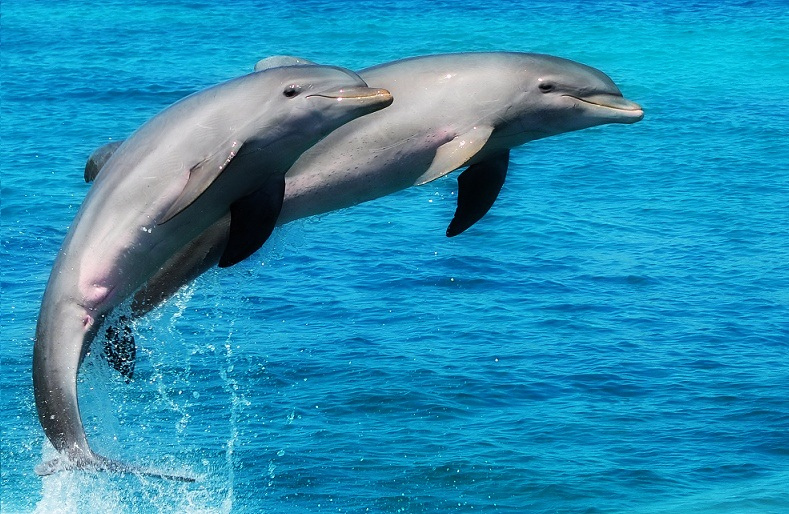
\includegraphics[height=2.2cm]{dolphin.jpg}
					\end{minipage}
				}
				\subfigure{
					\begin{minipage}{3cm}{(b) giraffe}
					\centering 
					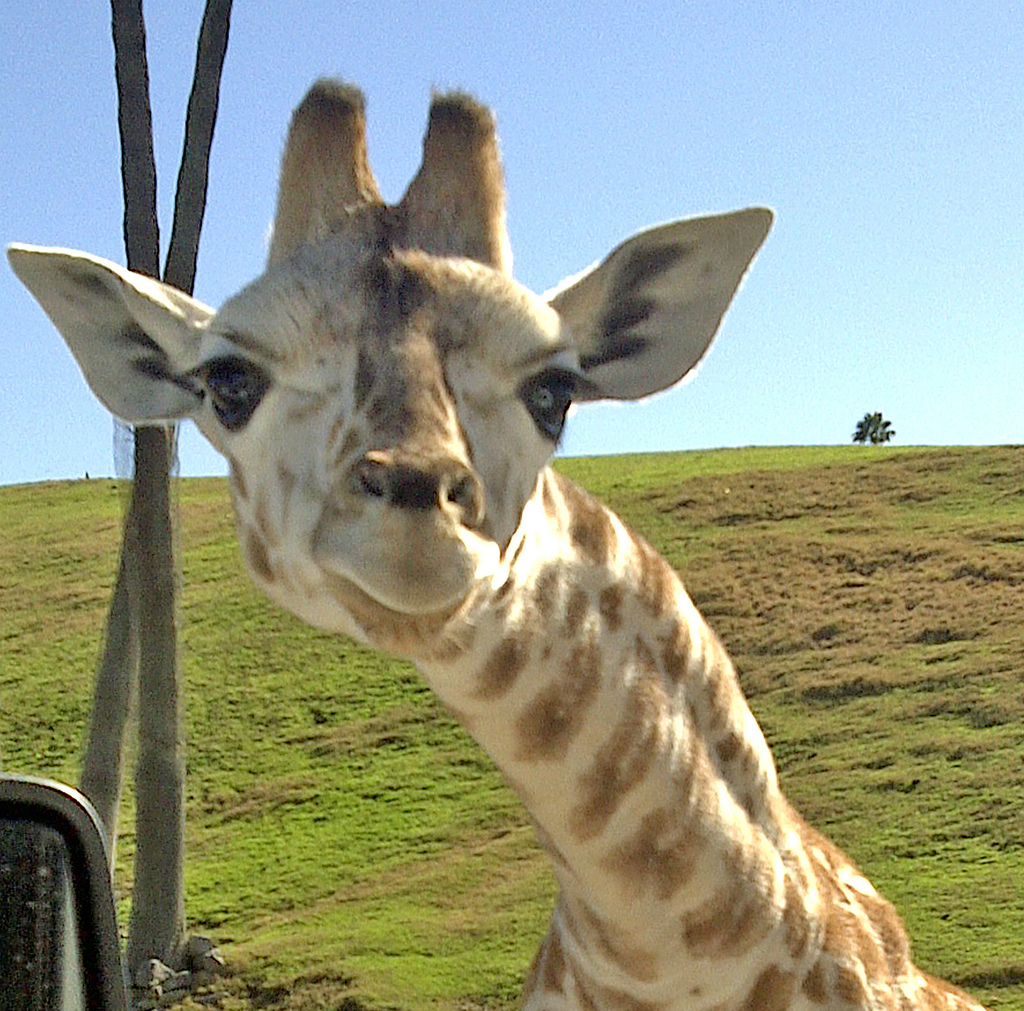
\includegraphics[height=2.2cm]{giraffe.jpg}
					\end{minipage}
				}
				\subfigure{
					\begin{minipage}{3cm}{(c) rabbit}
					\centering 
					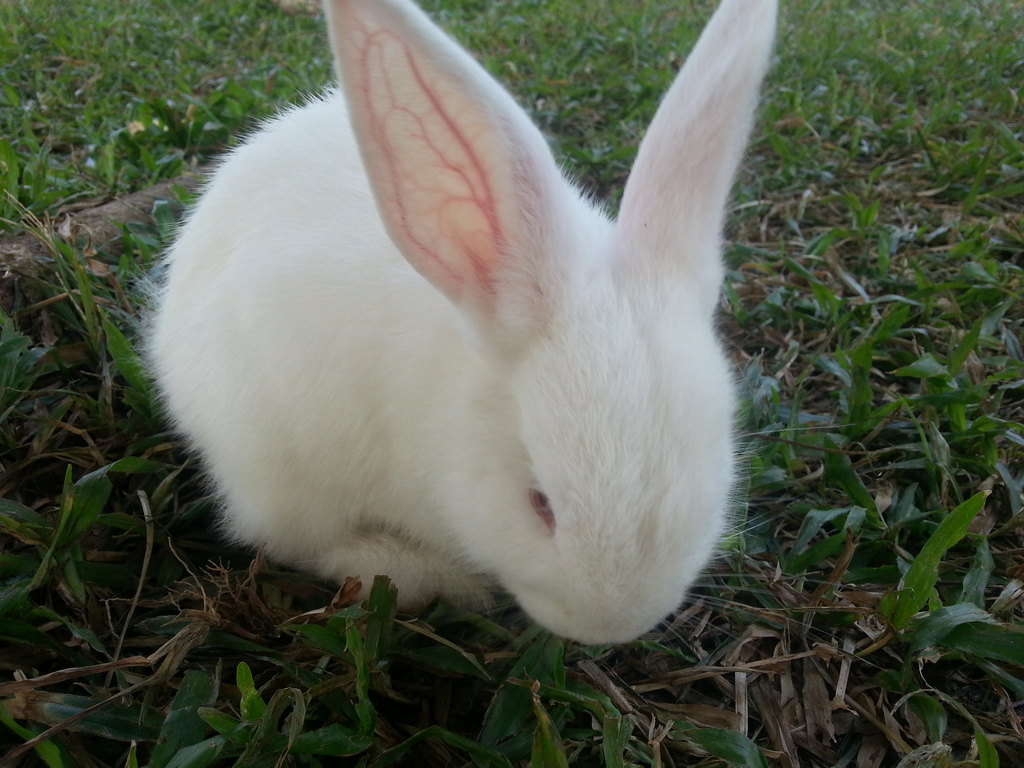
\includegraphics[height=2.2cm]{rabbit.jpg}
					\end{minipage}
				}
				\subfigure{
					\begin{minipage}{3cm}{(d) sheep}
					\centering 
					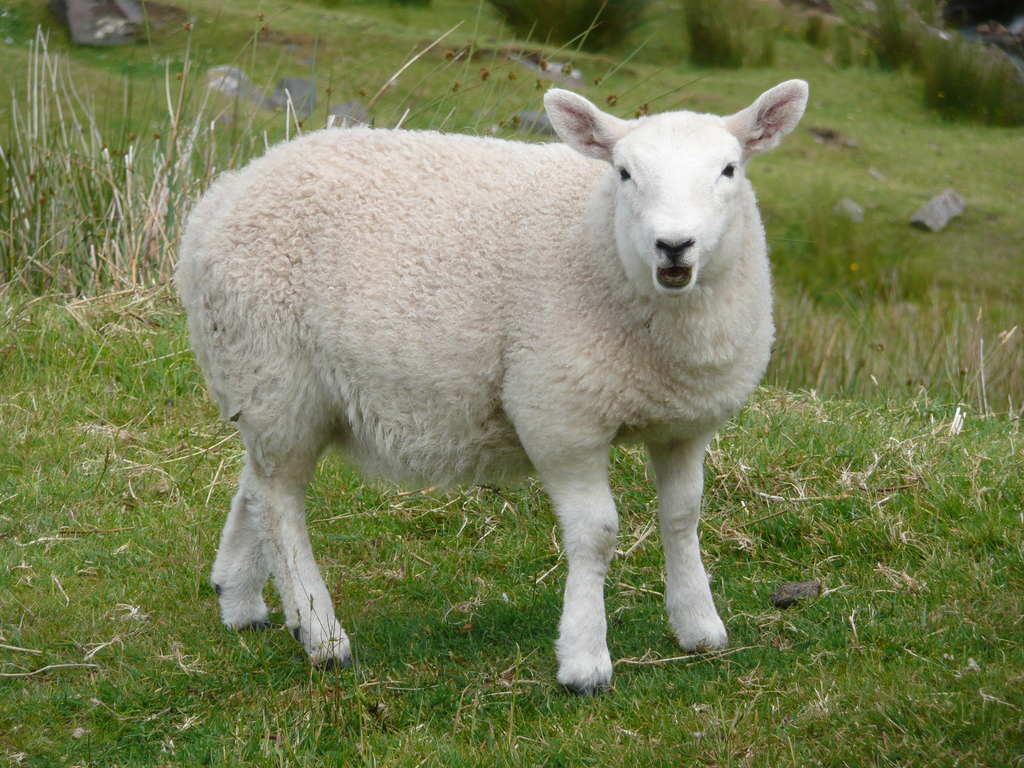
\includegraphics[height=2.2cm]{sheep.jpg}
					\end{minipage}
				}
				\caption{Images from 4 different classes.}\label{image}
			\end{figure}

\section{Methods} 
\subsection{Weak Classifier based on SIFT}
First of all, SIFT features is the most difficult one to deal with, because the number of feature points varies from one to another image, and the dimension of features is very high. There may be hundreds of feature points in a image after filtering, and each feature point is a 128-dimensional vector. So, the first step is reducing the dimension of feature points to 40 by PCA, because the first 40-dimensional components takes the majority for any image's feature points. Fig. \ref{pca} shows the average percentage of each dimension's component, which 
\begin{figure}[H]
				\centering
				\subfigure{
					\begin{minipage}{8cm}
					\centering 
					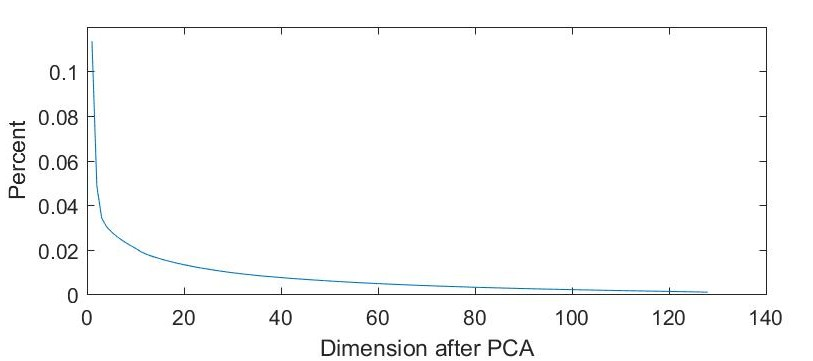
\includegraphics[height=4cm]{percent.jpg}
					\end{minipage}
					}
				\caption{The average percentage of each dimension's component of the sheep class.  }\label{pca}
\end{figure}
 \noindent is sampled from the sheep class. This step is based on the idea of PCA-SIFT but not quite same. Suppose $\{\mathbf{x}_{ij}\}^{n_j}_{j=1} \in \mathbb{R}^{128}$ are $n_j$ SIFT feature points extracted from image $i$, this step equals to solve the problem:
\begin{align}
	&\min_{e_1,e_2\dots  e_{40}}\sum\limits_{j=1}^{n_j} \|\mathbf{x}_{ij} - \mathbf{m} - \sum\limits_{k=1}^{40}\mathbf{e}_ka_{jk}\|^2\\
	s.j.& \|\mathbf{e}_1\|^2 = \|\mathbf{e}_2\|^2 = \dots = \|\mathbf{e}_{40}\|^2 = 1
\end{align}
The solution to this problem is:
\begin{align}
	\mathbf{m}& = \frac{1}{n_j}\sum\limits_{j=1}^{n_j}\mathbf{x}_{ij}\\
	a_{jk}& = \mathbf{e}_{k}^T(\mathbf{x}_{ij} - \mathbf{m})
\end{align}
And $\mathbf{e}_1,\mathbf{e}_2,\dots \mathbf{e}_{40}$ are the eigenvectors corresponding to the top 40 eigenvalues of $(\mathbf{X}_i-\mathbf{m})(\mathbf{X}_i-\mathbf{m})^T$, while $\mathbf{X}_i = [\mathbf{x}_{i1}\ \mathbf{x}_{i2}\ \dots \ \mathbf{x}_{in_j}]$.

Therefore, the feature after reduction is:
\begin{equation}
	\hat{\mathbf{X}}_i = [\mathbf{e}_1\ \mathbf{e}_2\ \dots\ \mathbf{e}_{40}]^T (\mathbf{X}_i-\mathbf{m}),
\end{equation}
while $\hat{\mathbf{X}}_i = [\hat{\mathbf{x}}_{i1}\ \hat{\mathbf{x}}_{i2}\ \dots \ \hat{\mathbf{x}}_{in_j}]$.

After dimension reduction, all feature points extracted from the training set should be put into the bag of words model together, which forms a set $\{\hat{\mathbf{x}}_{ij}|1\leq i \leq Nc, 1\leq j \leq n_i\}$. $c$ is the number of classes, $N$ is the number of images in each class (Suppose the numbers are same for the sake of clarity), and $n_i$ is the number of feature points in the image $i$. To divide these points in $K$ clusters, we want the sum of residual sum of squares is the least:
\begin{align}
	&\min_{C_1,C2,\dots C_K}\sum\limits_{m=1}^{K} \sum\limits_{\hat{\mathbf{x}}_{ij}\in C_m} \|\hat{\mathbf{x}}_{ij} - \mathbf{y}_m  \|^2\\
	s.j.\ &C_i\cap C_j = \varnothing\ \forall i,j \in \{1,2,\dots K\}, i \not= j\\
	&C_1\cup C_2 \cup \dots C_K = \{\hat{\mathbf{x}}_{ij}\},
\end{align}
while $C_1$ to $C_K$ are clusters and $\mathbf{y}_m$ is the representative point for cluster $C_m$. The constraints make sure that every points can be and only be assigned to one cluster. When the objective function gets minimum its derivative equals to zero:
\begin{equation}
	\mathbf{y_m} = \frac{1}{n_m} \sum\limits_{\hat{\mathbf{x}}_{ij}\in C_m} \hat{\mathbf{x}}_{ij},
\end{equation}
while $n_m$ is the number of points in the cluster $m$, and $\mathbf{y}_m$ is the mean of this cluster.

\begin{figure}[H]
				\centering
				\subfigure{
					\begin{minipage}{8cm}
					\centering 
					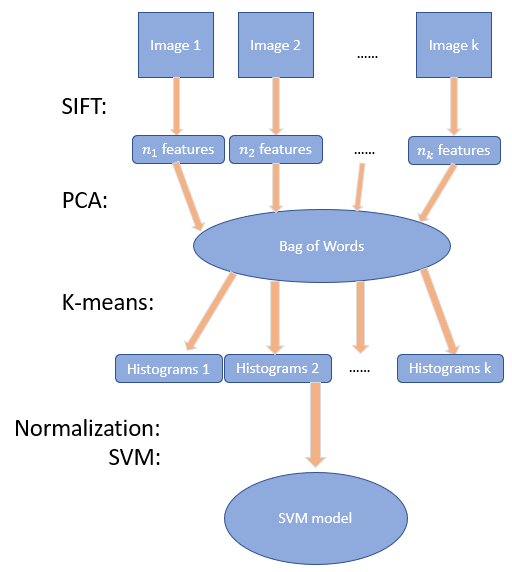
\includegraphics[height=7cm]{sift.jpg}
					\end{minipage}
					}
				\caption{ The flow chart of the weak classifier based on SIFT algorithm. SIFT features extracted from images will be reduced to 40 dimensions firstly, then put together to construct the bag of words model. After that, use K-means to cluster these feature points and count, proposing to convert feature points to histogram vectors. The final step is building the OVA SVM model. }\label{sift}
			\end{figure}

Unfortunately, it's a NP-hard problem and we can not guarantee an optimal solution. K-means algorithm is monotonically decreasing, which moves the cluster centers around in space in order to minimize RSS, and we can only prove it will eventually arrive at a local minimum. Several effective heuristics can be used to improve the results of K-means algorithm, including (i)  excluding outliers from the training set; (ii) trying out multiple starting points and choosing the clustering with lowest $RSS$; (iii) obtaining initial cluster centers from another method such as hierarchical clustering \cite{proving}.

The number of clusters $K$ can not be too large or too small. In fact, if there are $n$ points in the model, $K = \sqrt{n}$ is the best choice\cite{knn}. When the cluster centers are determined, feature points of each image can be assigned to these clusters according to the Euclidean distances between feature points and cluster centers. For the image $i$, a histogram vector $\mathbf{z}_i = [z_{ij}] \in \mathbb{R}^{K}$ counts the distribution of feature points, while $z_{ij}$ represents the number of feature points assigned to the cluster $j$ in the image $i$. Because the number of feature points is different from one to another image, the histogram vector need to be normalized:
\begin{equation}
	\hat{\mathbf{z}}_{i} = \frac{\mathbf{z}_{i}}{n_i},
\end{equation}
while $n_i = \sum\limits_{j=1}^{K}z_{ij}$. By these steps, an image can be transformed to a fixed-length vector.

The last step on this weak classifier is using one-versus-all (OVA) SVM\cite{ova} to classify the training set. Because the dimension of features $\hat{\mathbf{z}}$ is much bigger than the number of classes, linear kernel is enough for this problem. Suppose there are $c$ classes $\{1,2,\dots c\}$, $c$ binary classifiers are needed totally. For the $m_{th}$ binary SVM classifier, the training set is $\{[\hat{\mathbf{z}}_i, g(y_i,m)]\}_{i=1}^{Nc}$, while $y_i$ is the label of image $i$ and $g(y_i , m)$ is a logical function representing the label of $\hat{\mathbf{z}}_i$. In this training set, $g(y_i,m)=1$ if $y_i = m$ otherwise $-1$.  Images in class $m$ are regarded as the positive samples and images in other class are regarded as the negative samples. Taking outliers and noises into account, the optimization problem is:
\begin{align}
	\min_{\mathbf{w},b} &\ \frac{1}{2}\mathbf{w}^T\mathbf{w} + C \sum\limits_{i=1}^{Nc}\xi_i\\
	s.j.\ & g(y_i , m)(\mathbf{w}^T\hat{\mathbf{z}}_i+b)\geq 1-\xi_i\\
	& \xi_i\geq 0
\end{align}
The dual problem is:
\begin{align}
	\max  \sum\limits_{i=1}^{Nc}a_i - &\frac{1}{2}\sum\limits_{i=1}^{Nc}\sum\limits_{j=1}^{Nc}a_ia_jg(y_i , m)g(y_j,m)\hat{\mathbf{z}}_i^T\hat{\mathbf{z}}_j\\
	 s.j. &\ 0\leq	a_i\leq C\\
	 & \sum\limits_{i=1}^{Nc}a_ig(y_i, m) = 0
\end{align}
The problem can be solved by SMO and KKT conditions. Repeat $c$ times to get classifiers 
\begin{equation}
	h_m(\mathbf{z}) = \frac{\mathbf{w}_m^T\mathbf{z}+b_m}{\|\mathbf{w}_m\|},
\end{equation}
while $y = \mathbf{w}_m^T\mathbf{x}+b_m$ is the hyperplane and the absolute value of $h_m(\mathbf{z})$ is the distance between $\mathbf{z}$ and the hyperplane.

For a new sample $\mathbf{z}$ from the test set, the possibility that whether $\mathbf{z}$ belongs to class $m$ can be evaluated by the stand logistic function $f_m(\mathbf{z}) = \frac{1}{1+e^{-h_m(\mathbf{z})}} $. $\mathbf{z}$ should be classified to the class which gets the highest possibility:
\begin{align}
	y =& \argmax_{m \in \{1\dots K\}} f_m(\mathbf{z})\\
		= & \argmax_{m \in \{1\dots K\}} h_m(\mathbf{z})
\end{align}

The entire procedure of the weak classifier based on SIFT is shown in Fig. \ref{sift}. 

\subsection{Combining different features by AdaBoost}
It's more easier to deal with other two feature extraction algorithms, LBP and HOG, because they are aimed at the whole picture and can be converted to histogram vectors directly. OVA SVM is also used to as the finial step. As a result, we have three weak classifiers $H_1(i)$, $H_2(i)$, and $H_3(i)$ separately based on SIFT, LBP and HOG algorithms. The linear combination of these weak classifiers can be represented as:
\begin{equation}
	H(i) = sign(\sum\limits_{m=1}^{3}a_mH_m(i))
\end{equation}
\begin{figure}[H]
				\centering
				\subfigure{
					\begin{minipage}{8cm}
					\centering 
					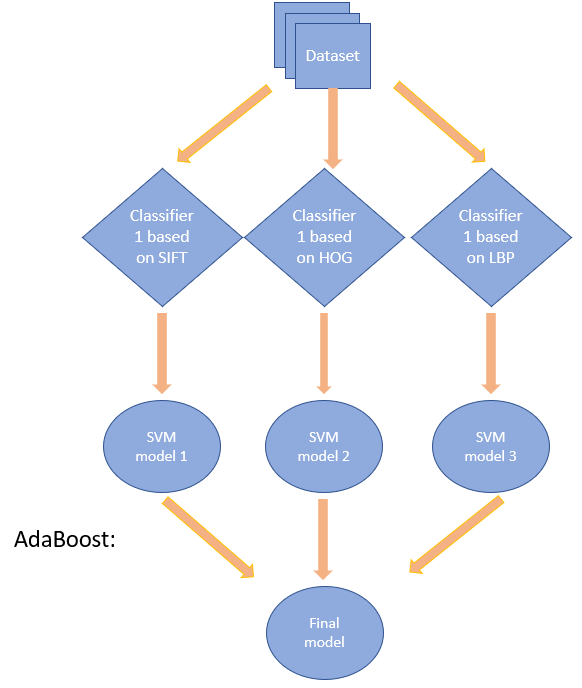
\includegraphics[height=7cm]{all.jpg}
					\end{minipage}
					}
				\caption{ The flow chart of the whole algorithm. From the dataset three kinds of features can be extracted. Based on these features, OVA SVM models are built separately. Finally, these models are combined by AdaBoost. }\label{all}
			\end{figure}

To get the best classifier, the exponential loss function is used because we want the loss is higher when a prediction is wrong and the loss is lower when a prediction is correct:
\begin{align}
	\mathcal{L} & = \sum\limits_{i=1}^{Nc}exp(-\sum\limits_{m=1}^{3}a_mg(y_i,H_m(i)))\\
\end{align}
while $g(y_i,H_m(i))$ represents the result of image $i$ given by the classifier $m$ is correct(1) or not(-1). As the combination of some base $e$ exponential functions, the loss function is convex. Suppose we have known the former $j-1$ weights ($j-1$ can equal to zero), and define two set $W_c = \{i|g(y_i,H_j(i)) = 1\}$ and $W_e = \{i|g(y_i,H_j(i)) \not= 1\}$, for the $j_{th}$ classifier we have\cite{ada}:
\begin{align}
 	\mathcal{L} & = \sum\limits_{i=1}^{Nc}C(i)exp(-a_mg(y_i,H_m(i)))\\
 	& = \sum\limits_{i \in W_c}C(i)e^{-a_m} +\sum\limits_{i\in W_e}C(i)e^{a_m}
 \end{align}
 while $C(i) = exp(-\sum\limits_{j=1}^{m-1}a_jg(y_i,H_j(i)))$ , and $C(i) = 1$ if $m-1 = 0$.
 When the objective function achieves the minimum:
 \begin{align}
 	\frac{\partial{\mathcal{L}}}{a_m} & = 0\\
 	a_m & = \frac{1}{2}ln(\frac{\sum\limits_{i\in W_c}C(i)}{\sum\limits_{i\in W_e}C(i)})
 \end{align}
The entire procedure of the whole classifier is
shown in Fig. \ref{all}. 

\section{Model Evaluation} The dataset will be divided into training set and test set with a ratio of 4:1. 5-fold cross-validation is used to guarantee models' generalization ability. The training and test process will be repeated 5 times and results will be averaged. Confusion matrix will be used to exhibit the quality of models, but the top-1 accuracy is the most important evaluation. The model combined three different features will be compared with models only using SIFT, LBP, or HOG in turn. It would be expected that the top-1 accuracy of the former model will be higher than that of any other model. 

\section{algorithm}
\begin{algorithm}
			
			\begin{algorithmic}[1]
			\REQUIRE The dataset 
			\ENSURE A classification model
			\STATE Split the dataset into 5 equal-sized subsets $s_1$ to $s_5$.
			\FOR {j = 1 to 5}
			\STATE Choose $s_j$ as the test test and other four subsets as the training set.
			\STATE Extracted SIFT, LBP and HOG features from the training set.
			\STATE Reduce the SIFT features to 40 dimension.
			\STATE Construct the bag of words model, use K-means to cluster SIFT features and calculate distribution histograms.
			\STATE Calculate distribution histograms of LBP and HOG features.
			\STATE Construct 3 weak classifiers $H_{j1}(i)$, $H_{j2}(i)$ and $H_{j3}(i)$ by one-versus-all SVM separately based on different feature histograms.
			\STATE Combine the three classifiers by AdaBoost $\rightarrow\ H_j(i)$ 
			\ENDFOR
			\STATE $H(i) = sign(\sum\limits_{j = 1}^{5}H_j(i))$
			\RETURN The classification model $H(i)$
			\end{algorithmic}
			\end{algorithm}
	


\section{Conclusion} 
Image classification occupies an important place in computer vision in the field of computer vision all the time. Compared to dedicating to the classifier itself, pay more attention on features extracted from images may be a new useful idea. It applies equally to some other high-performance image classification algorithms, such as CNN and ResNet in the field of deep learning.
In the future paper we hope to present persuasive results to support our conclusion.



\begin{thebibliography}{00}
\bibitem{sift}D. Lowe, “Object recognition from local scale-invariant features,” in \emph{ICCV}, 1999.
\bibitem{hog} N. Dalal and B. Triggs, ``Histograms of oriented gradients for human detection,'' in \emph{CVPR}, 2005.
\bibitem{lbp} DC. He and L. Wang, "Texture Unit, Texture Spectrum, And Texture Analysis", in \emph{IEEE Transactions on Geoscience and Remote Sensing}, vol. 28, pp. 509 - 512, 1990.
\bibitem{dataset}  Y. Xian, C. H. Lampert, B. Schiele, and Z. Akata, ``Zero-Shot Learning - A Comprehensive Evaluation of the Good, the Bad and the Ugly," in \emph{CVPR}, 2017.
\bibitem{proving} C. D. Manning, P. Raghavan, and H. Schütze, ``Introduction to information retrieval,'' New York: Cambridge University Press, 2009, pp.360-365.
\bibitem{knn} X. Wang,``A fast exact k-nearest neighbors algorithm for high dimensional search using k-means clustering and triangle inequality,'' \emph{The 2011 International Joint Conference on Neural Networks}, 2011.
\bibitem{ova} C. Hsu and C. Lin, "A comparison of methods for multiclass support vector machines," in \emph{IEEE Transactions on Neural Networks}, vol. 13, no. 2, pp. 415-425, Mar 2002.
\bibitem{ada} R. Rojas, ``Adaboost and the super bowl of classifiers a tutorial introduction to adaptive boosting,'' \emph{Freie University, Berlin, Tech. Rep.}, 2009.
\end{thebibliography}

\end{document}
